\chapter{Эмоциональные состояния на уровне нейробиологических процессов.}
\label{chap:theoretical_development}

Исследование эмоциональных вычислений как поиск моделей, объясняющих эмоции, начиналось в областях психологии, нейропсихологии и философии. Эволюционная теория происхождения эмоций Ч. Дарвина объясняла эмоции как приспособительные механизмы, жизненно важные для адаптации организма к условиям жизни — неважно, человека или животного. Д. Пейпец выдвигал гипотезу о единой системе, объединяющей структуры мозга, участвующие в формировании эмоций, — позже она получила название лимбической системы. Исследования Ф. Барда, подкрепленные данными физиологии, свидетельствовали, что физиологические проявления и субъективные переживания эмоциональных процессов происходят одновременно, благодаря расщеплению возбуждающего нервного импульса в таламусе. Двухфакторная теория эмоций С. Шехтера разделяла эмоцию на эти же два компонента: физиологическое возбуждение и его когнитивную интерпретацию.


Десятилетиями нейробиологи публиковали результаты экспериментов о том, нейроны какого типа и в какой части мозга проявляют активность, в зависимости от состояния организма, в том числе и эмоционального состояния. Эти многочисленные данные собраны и обобщены доктором психиатрии Хьюго Левхеймом, который предложил на их основе новую трёхмерную модель эмоций.\cite{lovheim2012} Базовые эмоции (аффекты), объясняемые в его работе нейробиологически, берутся из психологической модели Сильвана Томкинса.\cite{tomkins1962, tomkins1963, tomkins1991} Теория аффектов Томкинса разделяет 9 «первичных» эмоций (наблюдаемых с рождения) на категории и соединяет каждую с типичным физиологическим проявлением, позой, выражением лица. Например, злость — покрасневшее лицо, сжатые челюсти, сдвинутые брови. Из этих 9 эмоций Левхейм не стал вводить в модель эмоцию реакции на неприятный запах, остальные 8 включены и присутствуют на рисунке ~\ref{fig:cube_0}.


\begin{figure}
	\centering
	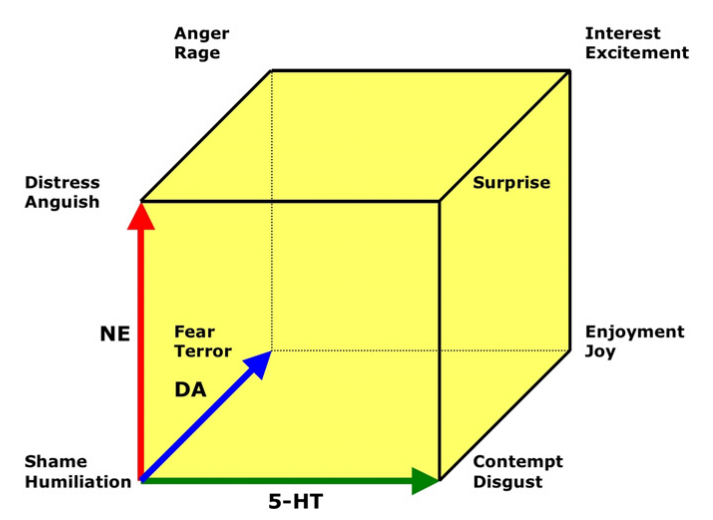
\includegraphics[width=\linewidth]{cube_0}
	\caption{Модель Левхейма, задающая трёхмерное пространство эмоций через нейромедиаторы серотонин, дофамин и норадреналин.}
	\label{fig:cube_0}
\end{figure}


Тремя измерениями модели Левхейма являются уровни концентрации моноаминовых нейромедиаторов серотонин, дофамин и норадреналин — минимально необходимое количество для того, чтобы специально упрощённая модель оставалась реалистичной. Нейромедиаторы это биологически активные химические вещества,  контролирующие процессы, происходящие между нейронами. Системы названных моноаминовых нейромедиаторов эволюционно сохраняются в различных организмах, они контролируют поведение как людей, так и крыс, лобстеров, пустынной саранчи и др. Эти системы обеспечивают гибкость поведения и способность адаптироваться к постоянно изменяющейся окружающей среде, сами по себе также являются динамичными.\cite{Benarroch17112009}


Нейронная активность может модифицироваться и перенастраиваться, когда концентрация нейромедиатора повышается из-за активности конкретных зон мозга (например, голубоватого пятна, в случае норадреналина). Нейромедиатор разносится по другим областям мозга, где влияет на многочисленные рецепторы подходящего типа. Это может усиливать или ослаблять связь между нейронами, если связь также была активна совсем недавно (эффект собаки Павлова), менять свойства нейронов.\cite{parsingreward} У таких нейромодулирующих систем существуют анатомические привилегии широкого доступа к многим областям нервной системы, и они идеально расположены для регулирования всех процессов обработки и хранения информации в мозге. Нейромодулирующие системы принимают активное участие в работе двигательных, чувственных и когнитивных функций.\cite{zarrindast} Их роль в работе мозга настолько велика, что, несмотря на внушительное количество уже имеющихся экспериментальных данных, вопросы взаимодействия нейромедиаторов друг с другом, точного механизма их функционирования и прочие остаются открытыми, требующими длительного дальнейшего изучения.


На рисунке 1 зелёная ось «5-HT» обозначает уровень концентрации нейромедиатора серотонин. В человеческом организме серотонин отвечает за регуляцию поведения, аппетит, обучение, общение — за всё, что делают в спокойном состоянии. Низкий уровень серотонина влечёт сонливость, высокий уровень серотонина повлечёт за собой половое влечение,  быстрое переваривание пищи, чувство эйфории и ощущение непобедимости. Серотонин работает над уверенностью в себе, особенно после верно принятых решений, и над контролем агрессии. В точке, где концентрация серотонина максимальна, а остальных минимальна, расположена эмоция сытости/отвращения/презрения.


Красная ось «NE» - уровень концентрации нейромедиатора норадреналин, или норэпинефрин. Уровень его концентрации повышается в ответ на стрессовые ситуации, раздражители и на всё новое, либо неожиданное. Высокий уровень деятельности норадреналина вызывает повышение бдительности и скорости реакции, концентрацию внимания, улучшение обработки сенсорных входов, повышение уровня возбуждения. В точке, где концентрация норадреналина максимальна, а остальных миинимальна, расположена эмоция страдания/отчаяния. Мозг испытывает ощущение бедствия, когда произошло что-то непоправимое или болезненное, и максимально сконцентрирован на этом событии.


Синяя ось «DA» - уровень концентрации нейромедиатора дофамин. Он отвечает за наслаждение и удовольствие от выполненного дела, вкусной еды, приятных ощущений, даёт ощущение награды, таким образом закрепляя важные для выживания и благосостояния действия. Дофамин используется мозгом для оценки действий и мотивации, а также для активации моторных функций. В точке, где его концентрация максимальна, а остальных минимальна, находится эмоция «страх».


В точке, где концентрация каждого нейромедиатора минимальна, располагается эмоция «стыд», когда нет ни сфокусированности внимания, ни чувства удовлетворения, ни уверенности в себе. Повышенные уровни дофамина и норадреналина влекут «ярость», серотонина и норадреналина - «удивление», дофамина и серотонина — спокойное «удовольствие». Высокий уровень концентрации всех трёх нейромедиаторов в модели Левхейма связан с эмоцией активной «заинтересованности», «увлеченности».


Отображение клеточных реакций на вычислительный процесс должно быть осуществлено так, чтобы при удалении всей биохимии, отсутствии настоящих моноаминов и белков удалось сохранить роли нейромедиаторов в системе. Были предложены следующие аналогии \cite{talanov2014}, зафиксированные на рисунке ~\ref{fig:cube_1}:
\begin{itemize}
\item Серотонин регулирует вычислительную мощность и выделяет постоянную память для хранения данных. Поскольку серотонин участвует в обучении и накоплении опыта, то результаты принятых решений, во-первых, нужно запомнить в качестве удовлетворительного или стыдного опыта (выделить для них память). Во-вторых, в зависимости от результата, за решением следует прилив сил и уверенности (мощности) или их упадок.
\item Норадреналин отвечает за перераспределение вычислительных процессов и выделение оперативной памяти. Это соответствует переключению внимания в организме живого существа: мыслительные процессы тоже перераспределяются, чтобы полностью сконцентрироваться на том, что привлекло внимание.
\item Дофамин, во-первых, выделяет постоянную память для хранения данных, как и серотонин — поскольку тоже участвует в обучении. Во-вторых, поскольку дофамин сильно влияет на мотивацию, ???????????????????????????.
\end{itemize}


\begin{figure}
	\centering
	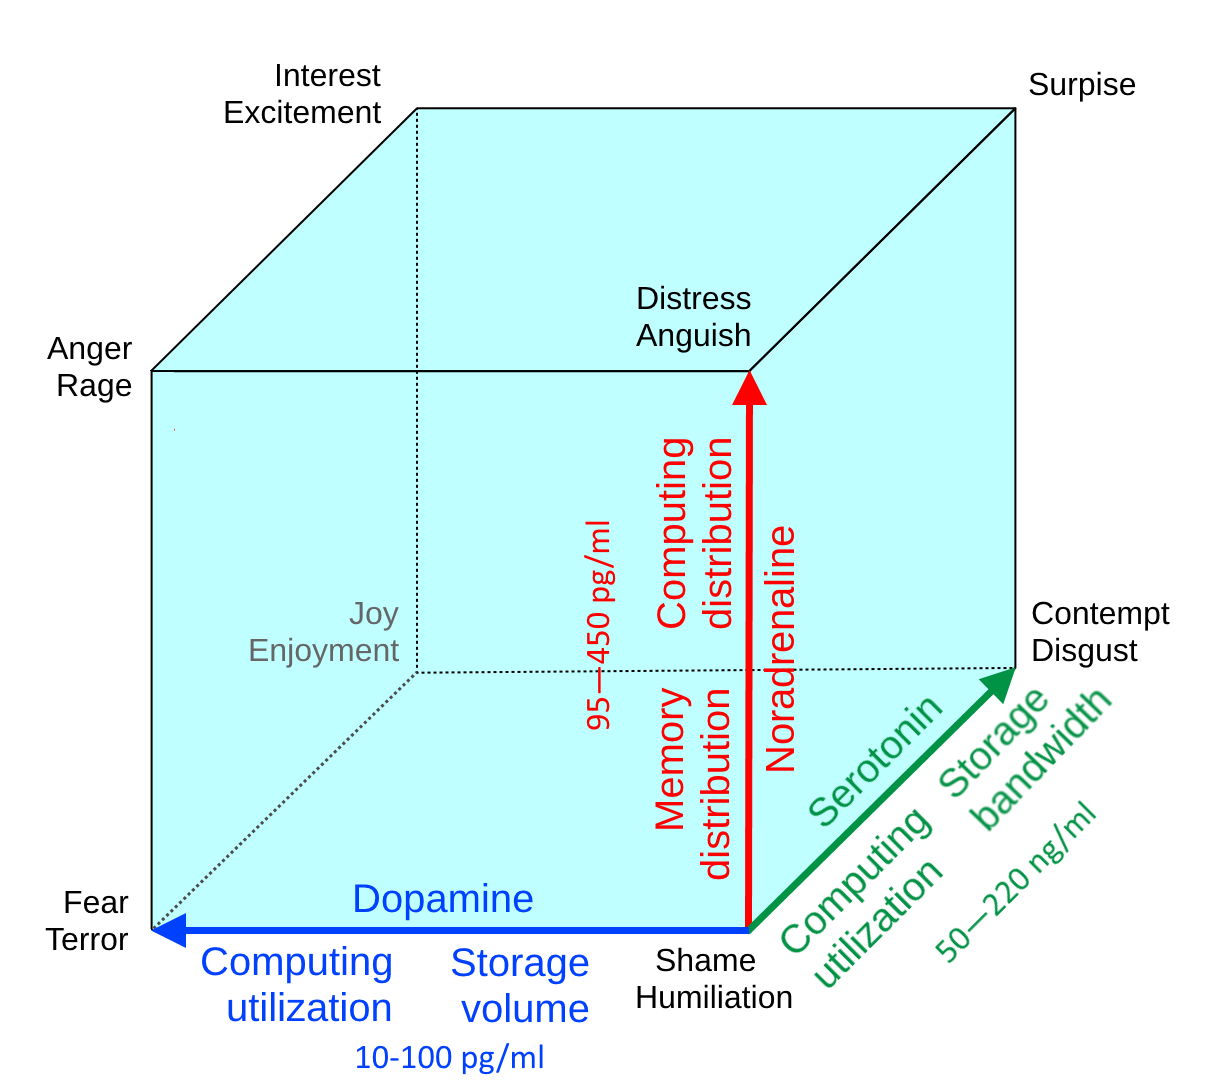
\includegraphics[width=\linewidth]{cube_1}
	\caption{Дополненная модель Левхейма. Проведение аналогии роли нейромедиаторов с вычислительными процессами.}
	\label{fig:cube_1}
\end{figure}
